\documentclass[pdf,aspectratio=169]{beamer}
\usepackage[]{hyperref,graphicx,siunitx,lmodern,booktabs,tikz,tensor}
\usepackage{pgfplots, pgfplotstable}
\usepackage{pdfpc-commands}
\usepackage[mode=buildnew]{standalone}
\mode<presentation>{\usetheme{Astro}}

\graphicspath{ {../Images/} }

\sisetup{per-mode=symbol, group-separator={,}}
\usetikzlibrary{calc,intersections, decorations.pathmorphing,shadings,shapes.geometric}
%\tikzstyle{proton}=[circle, minimum size = 7mm, ball color=red, black,transform shape]
%\tikzstyle{neutron}=[circle, minimum size=7mm, ball color=gray, black, transform shape]
%\tikzstyle{gammaray}=[ultra thick, -latex, decorate, decoration={snake, post length=3mm}]


%preamble
\title{Life's Better the Milky Way}
\date{November 14, 2018}
\author{Jed Rembold}

\begin{document}
\renewcommand*{\theenumi}{\Alph{enumi}}

\begin{frame}{Announcements}
  \begin{itemize}
	\item Nothing due on Friday. Study up!
	\item I will not assign anything over Thanksgiving break
	\item Test 3 on Friday!
	  \begin{itemize}
		\item All study materials and solutions posted
		\item Same format as past tests
		\item Email me if you want to borrow a calculator!
	  \end{itemize}
	\item Polling: \url{rembold-class.ddns.net}
  \end{itemize}
\end{frame}

\begin{frame}{New Comet!}
	\begin{columns}
		\column{0.5\textwidth}
		\begin{center}
			\includegraphics[width=0.8\textwidth]{2018113_NewComet.jpg}
		\end{center}
		
		\column{0.5\textwidth}
		\begin{itemize}
			\item Found manually by amateur astronomer Don Machholz
			\item His 12th discovery!
			\item Orbit still being determined
			\item Estimated perihelion in late November to mid December
			\item Around magnitude 8
		\end{itemize}
		
	\end{columns}
\end{frame}

\begin{frame}{Review Question}
  Through some black magic (obviously), the Sun is converted into a black hole with mass equal to the Sun's current mass. Which of the following is true?
  \begin{enumerate}
	\item Earth's orbit starts to spiral slowly towards the black hole, owing to the black hole's increased gravity
	\item Earth's orbit travels straight toward the black hole (no spiral)
	\item Earth's orbit spirals away from the black hole, owing to an increase in the solar wind
	\item \alert<2>{Earth's orbit does not change}
  \end{enumerate}
\end{frame}

\begin{frame}{Portals across the Universe}
  \begin{itemize}
	\item Supermassive black holes actually have weaker tidal forces
	  \begin{itemize}
		\item Their size means you need to be further away from the singularity
	  \end{itemize}
	\item Could maybe cross without being spaghettified
	\item Rotating or charged black holes have bizarre properties
	\item Wormholes to other dimensions?
  \end{itemize}
\end{frame}

\begin{frame}{How do we find them?}

  \begin{itemize}
	\item Noting their orbital effects
	  \begin{itemize}
		\item Their huge mass makes an obvious effect on their surroundings
		\item Look for everything orbiting something that can't be seen!
	  \end{itemize}
	\item Gravitational Lensing
	  \begin{itemize}
		\item Light can be bent as it passes the black hole
	  \end{itemize}
  \end{itemize}
  \begin{center}
	\includegraphics[width=.5\textwidth]{ch14_grav_lensing.jpg}
  \end{center}
\end{frame}

\begin{frame}{LIGO!}
	\begin{itemize}
		\item Can now use gravity waves to look for energetic events from black holes!
			\begin{itemize}
				\item Swallowing of neutron star by black hole
				\item Merging of two black holes
			\end{itemize}
		\item Stretches are TINY!
			\begin{itemize}
				\item Like measuring differences in a human hair from here in Alpha Centauri!
			\end{itemize}
		\item Earth stretches and squeezes as the wave moves past us
	\end{itemize}
\end{frame}

%\begin{frame}{Understanding Check}
  %Which of the following is not true?
  %\begin{enumerate}
	%\item Approaching a supermassive black hole's event horizon is less likely to spaghetti-fy you than approaching a smaller black hole
	%\item The more massive a black hole, the greater the radius of its event horizon
	%\item Light shining out from objects near an event horizon is greatly redshifted
	%\item \alert<2>{Watching someone fall into a black hole only takes a split second, due to the extreme gravity}
  %\end{enumerate}
%\end{frame}

\fullFrameImageZoomedHorizontal{ch15_milkyway.jpg}

\begin{frame}{Origins}
  \begin{itemize}
	\item To the Greeks appeared as a ribbon of milk across the sky
	  \begin{itemize}
		\item Likely the source of its name
		\item Greek word for milk: galactose
	  \end{itemize}
	\item Galileo was the first to turn his telescope on it
	  \begin{itemize}
		\item Learned that it was composed of stars
		  \begin{quote}
			``The galaxy is, in fact, nothing but a collection of innumerable stars grouped together in clusters. Upon whatever part of it the telescope is directed, a vast crowd of stars is immediately presented to view. Many of them are rather large and quite bright, while the number of smaller ones is quite beyond calculation.''
			
			-Galileo Galilei, The Starry Messanger (1610)
		  \end{quote}
	  \end{itemize}
  \end{itemize}
\end{frame}

\begin{frame}{Shaping a Picture}
  \begin{itemize}
	\item Determining the shape of an object that one is \alert{interior} to can be tricky
	\item How would you estimate the size and shape of Collins, without leaving this room?
	  \begin{itemize}
		  \item<+-> We can't see through walls, so visible obstructions are a serious problem
		\item<+-> Exterior windows don't give us a view of the building
		  \begin{itemize}
			\item Must be on the edge?
		  \end{itemize}
		\item<+-> Interior window:
		  \begin{itemize}
			\item Portion of a hallway
			\item Doors indicating other rooms?
			\item Stairs indicating some height?
		  \end{itemize}
	  \end{itemize}
  \end{itemize}
\end{frame}

\begin{frame}{The Story of a Band}
  \begin{itemize}
	\item If the Milky Way appears as a band across the sky, what does that tell us?
	  \begin{itemize}
		\item See way more stars when looking in one direction than nearly any other
	  \end{itemize}
	\item The galaxy must be fairly flat
  \end{itemize}
  \begin{center}
	\begin{tikzpicture}[scale=1.25]
	  \pgfmathsetseed{1234567}
	  \foreach \p in {1,2,...,350}{
		\fill[inner color=yellow, outer color=orange] (rand*5.5,rand) circle (1pt);
	  }
	  \coordinate (earth) at (-1,0);
	  \node at (earth) {\includegraphics[width=3mm]{world.png}};
	  \def\dist{2}
	  \onslide<1>{\fill[orange, opacity=0.5] (earth) --+(-4:\dist) arc(-4:4:\dist) --cycle;}
	  \onslide<2>{\fill[orange, opacity=0.5] (earth) --+(86:\dist) arc(86:94:\dist) --cycle;}
	  \onslide<3>{\fill[orange, opacity=0.5] (earth) --+(176:\dist) arc(176:184:\dist) --cycle;}
	  \onslide<4>{\fill[orange, opacity=0.5] (earth) --+(266:\dist) arc(266:274:\dist) --cycle;}
	\end{tikzpicture}
  \end{center}
\end{frame}

\begin{frame}{Need a Larger Ruler}
  \begin{itemize}
	\item So how does one attempt to measure the galaxy?
	\item In the early 1800's, William and Caroline Herschel tried counting stars
	 \item They concluded:
	   \begin{itemize}
		 \item The Milky Way was 5 times as wide as it was thick
		 \item Sun was near the center
		 \item Had several branches
	   \end{itemize}
  \end{itemize}
  \begin{center}
	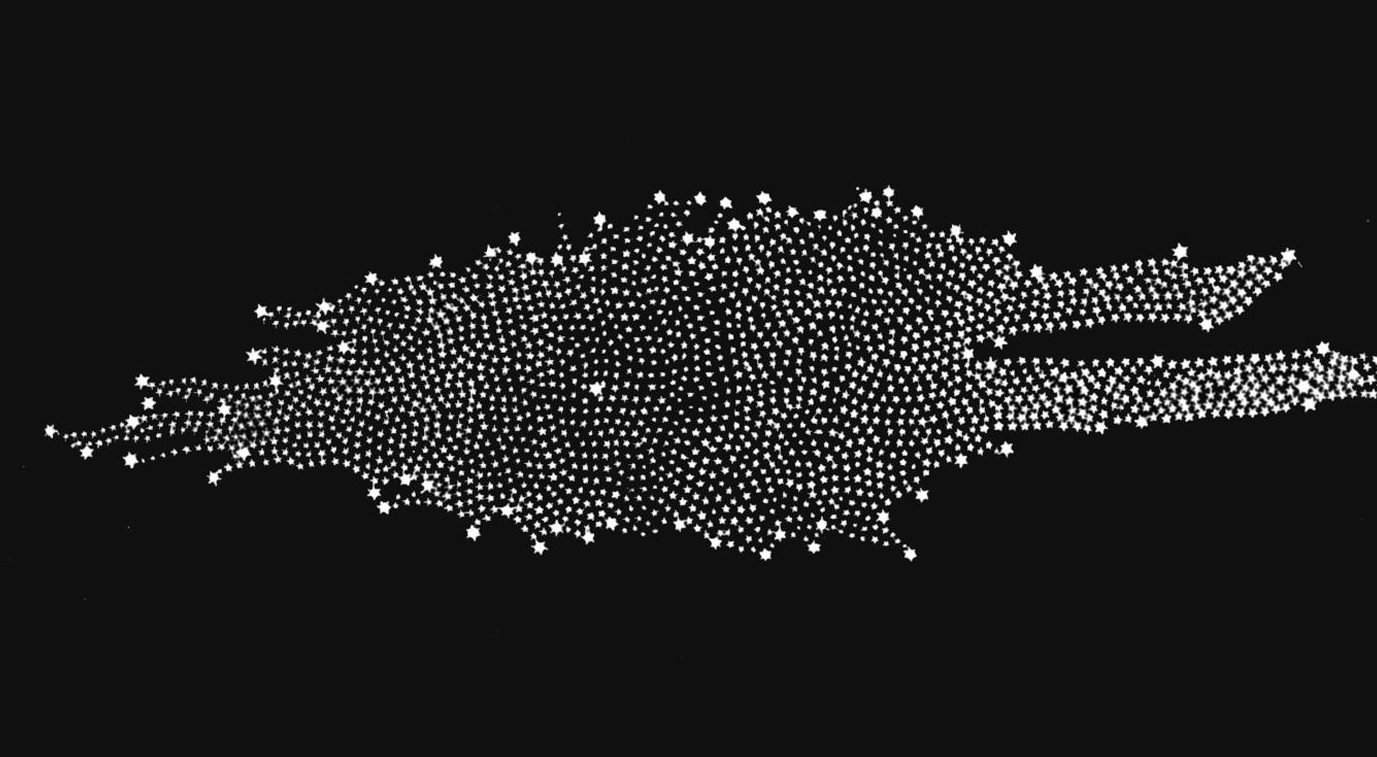
\includegraphics[width=.55\textwidth]{ch15_herschel.jpg}
  \end{center}
\end{frame}

\begin{frame}{What Went Wrong?}
  \begin{itemize}
	\item Herschel had no way of knowing about stellar distances
	  \begin{itemize}
		\item First parallax measurements were gotten 15 years after his death
	  \end{itemize}
	\item He also didn't realize it was impossible to ``see'' to the edge of the galaxy
	  \begin{itemize}
		\item Many stars would be too faint to see with his telescope
		\item Much of the galaxy is obscured by dust!
	  \end{itemize}
  \end{itemize}
  \begin{center}
	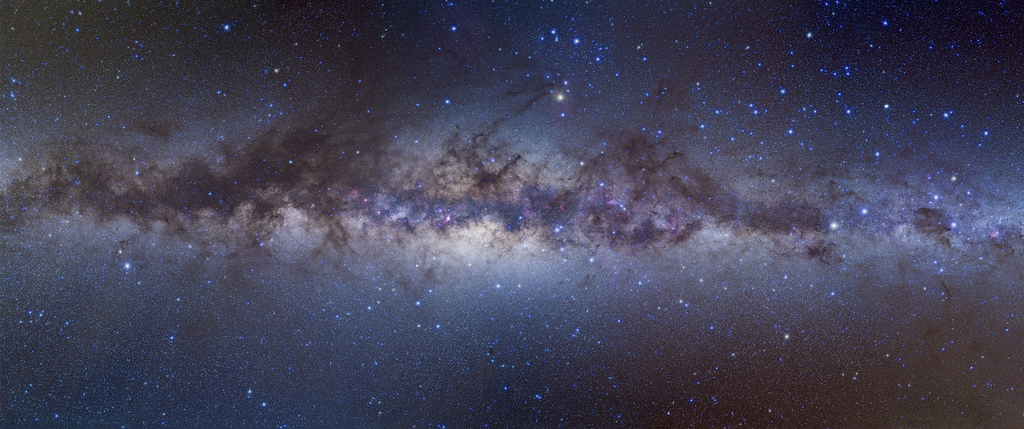
\includegraphics[width=.8\textwidth]{ch15_dustlanes.jpg}
  \end{center}
\end{frame}

\begin{frame}{Attempt Numero Dos}
  \begin{columns}
	\column{.4\textwidth}
	\begin{itemize}
	  \item Harlow Shapley attempted to use globular clusters
	  \item Globular clusters live mostly above or below the dust cloud
	  \item Many stars so brighter and easier to see
	  \item Findings:
		\begin{itemize}
		  \item Found a spherical distribution
		  \item Definitely not centered on the Sun
		\end{itemize}
	\end{itemize}
	\column{.6\textwidth}
	\begin{center}
	  \begin{tikzpicture}
		\begin{axis}[
			height=7cm,
			width=8cm,
			xlabel = Distance from Sun (kpc),
			ylabel = Distance from Sun (kpc),
		  ]
		  \addplot+[only marks, draw, color=cyan] table[x index=0, y index=1] {../Data/Shapley.csv};
		  \fill[inner color=yellow, outer color=orange] (axis cs: 0,0) circle (4pt);
		  \fill[red] (axis cs: 16,0) circle (2pt);
		\end{axis}
	  \end{tikzpicture}
	\end{center}
  \end{columns}
\end{frame}

\begin{frame}{Galactic Distances}
  \begin{itemize}
	\item Note most precise methods of determining shape rely on accurate distance measurements
	\item But we can only measure parallaxes for nearby stars\ldots
  \end{itemize}
  \begin{center}
	\begin{tikzpicture}[scale=.75,transform shape]
	  \node[outer sep=0pt, inner sep=0pt] at (0,0) {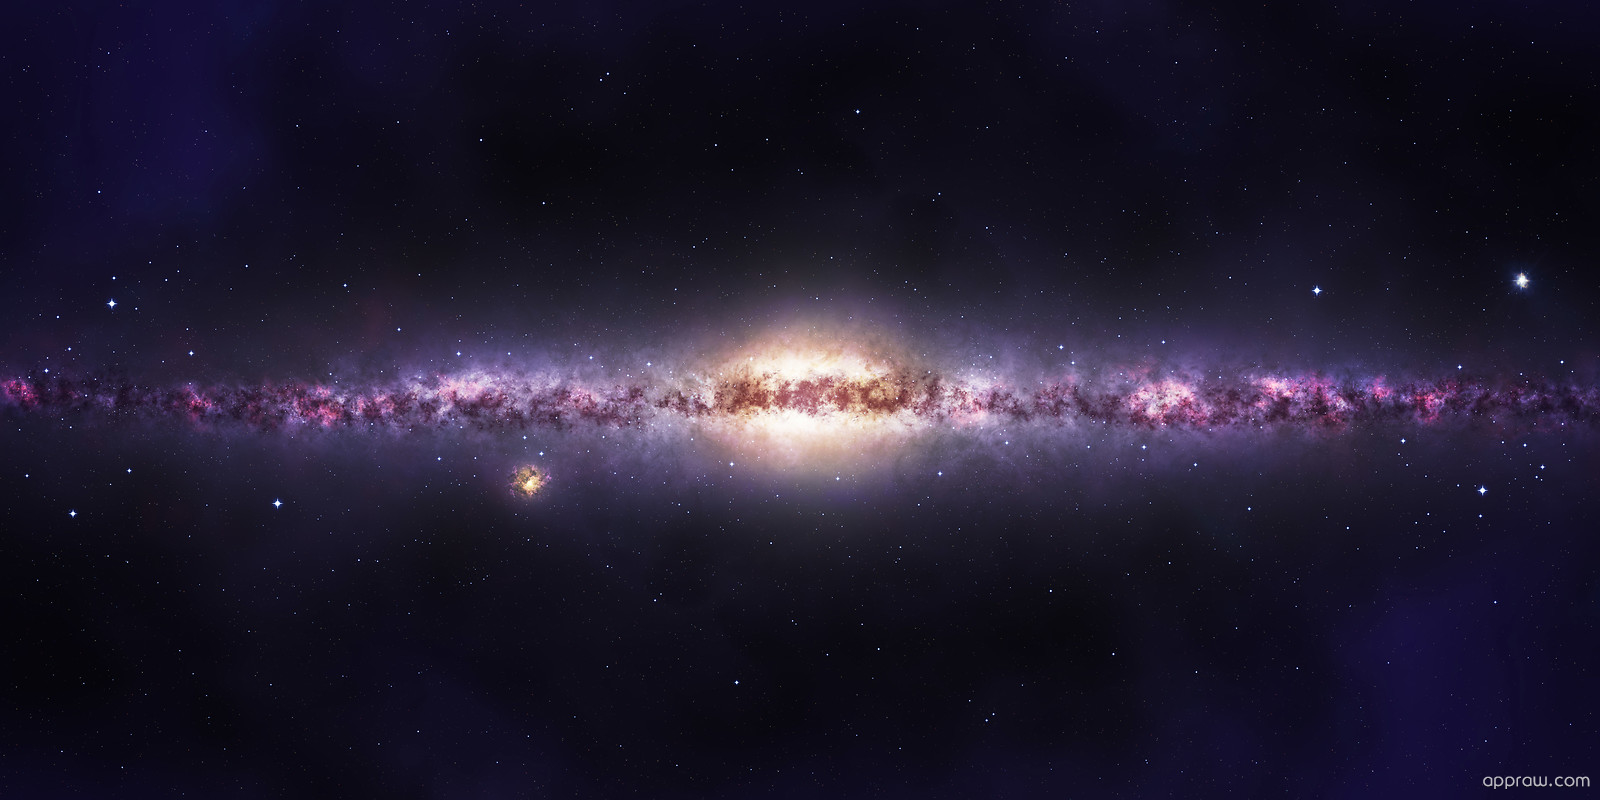
\includegraphics[width=\textwidth]{ch15_galaxy_side.jpg}};
	  \coordinate (star) at (-4,0);
	  \node[star, minimum size=3mm, inner color=yellow, outer color=orange, inner sep=0pt] at (star) {};
	  \draw<2>[cyan,dashed,very thick] (star) circle (2mm);
	  \draw<3>[orange,dashed,very thick] (star) circle (1);
	\end{tikzpicture}
  \end{center}
\end{frame}

\begin{frame}{Enter Cepheid Variables}
  \begin{columns}
	\column{.4\textwidth}
	\begin{itemize}
		\item Section 19.3
	  \item Giant Stars with very predictable pulsations
	\end{itemize}
	\column{.7\textwidth}
	\begin{center}
	  \begin{tikzpicture}
		\pgfplotsset{colormap={stars}{[0.1cm] color(0cm)=(blue); color(1.8cm)=(white); color(2.1cm)=(yellow); color(2.6cm)=(red); color(3cm)=(red!50!black)}}
		\hspace{-1cm}
		\begin{loglogaxis}[
			width=8.5cm,
			height=4cm,
			x dir = reverse,
			%xlabel = Temperature (K),
			%ylabel = Fraction of Sun's Luminosity,
			ticklabel style={font=\tiny},
			xtick = {3000, 6000, 10000, 25000},
			xticklabels = {3000,6000,10000,25000},
			colormap name= stars,
			xmin = 2000,
			xmax = 40000,
		  ]
		  \addplot[scatter, scatter src=-x, draw=black, only marks, mark size = 1pt] table[x index=0, y index=1] {../Data/HR_Data.csv};
		  \node[font=\scriptsize] at (axis cs: 10^4.5,10^-4) {O};
		  \node[font=\scriptsize] at (axis cs: 10^4.2,10^-4) {B};
		  \node[font=\scriptsize] at (axis cs: 10^3.95,10^-4) {A};
		  \node[font=\scriptsize] at (axis cs: 10^3.85,10^-4) {F};
		  \node[font=\scriptsize] at (axis cs: 10^3.7,10^-4) {G};
		  \node[font=\scriptsize] at (axis cs: 10^3.6,10^-4) {K};
		  \node[font=\scriptsize] at (axis cs: 10^3.4,10^-4) {M};
		\end{loglogaxis}
		%\draw<2>[cyan, ultra thick] (1.4,4.2) circle (1.5cm);
	  \end{tikzpicture}
	\end{center}
  \end{columns}
  \begin{center}
	\begin{tikzpicture}
	  \begin{axis}[
		  width=12cm,
		  height=4cm,
		  xlabel= Period (Days),
		  ylabel= {Apparent\\Magnitude},
		  ylabel style = {align=center},
		]
		\addplot[only marks, orange] table[x index=0, y index=1] {../Data/cepheid.csv};
	  \end{axis}
	\end{tikzpicture}
  \end{center}
\end{frame}

\begin{frame}{Time = Power!}
  \begin{columns}
	\column{.4\textwidth}
	\begin{itemize}
	  \item In 1912 Henrietta Leavitt noticed that Cepheid variables in the Small Magellanic Cloud:
		\begin{itemize}
		  \item Higher Luminosities
		  \item Had longer pulsation periods
		\end{itemize}
	  \item This gives us an easy method to find luminosities!
	  \item Which gives us distances!
	\end{itemize}
	\column{.6\textwidth}
	\begin{center}
	  \begin{tikzpicture}
		\begin{loglogaxis}[
		  width=8cm,
		  xlabel = Period (Days),
		  ylabel = Luminosity ($L_{\odot}$),
		]
		  \addplot[only marks, Red, mark=o, thick] table[x index=0, y index=1] {../Data/Type 2.csv};
		  \addplot[orange, only marks, mark=o, thick] table[x index=0, y index=1] {../Data/Type I.csv};
		  \addplot[cyan, only marks, mark=o, thick] table[x index=0, y index=1] {../Data/RR Lyrae.csv};
		  \node[orange] at (axis cs: 1,3e4) {Type I};
		  \node[Red] at (axis cs: 1,1e4) {Type II};
		  \node[cyan] at (axis cs: 1,4e3) {RR Lyrae};
		\end{loglogaxis}
	  \end{tikzpicture}
	\end{center}
  \end{columns}
\end{frame}

\begin{frame}{Understanding Check!}
 A Type I Cepheid variable star is measured with a pulsation period of 20 days. What is the star's maximum luminosity? 
  \begin{columns}
	\column{.3\textwidth}
	\begin{enumerate}
	  \item \num{10}$L_\odot$
	  \item \num{2000}$L_\odot$
	  \item \alert<2>{\num{10000}$L_\odot$}
	  \item \num{50000}$L_\odot$
	\end{enumerate}
	\column{.6\textwidth}
	\begin{center}
	  \begin{tikzpicture}
		\begin{loglogaxis}[
		  width=7cm,
		  xlabel = Period (Days),
		  ylabel = Luminosity ($L_{\odot}$),
		  grid=major,
		]
		  \addplot[only marks, Red, mark=o, thick] table[x index=0, y index=1] {../Data/Type 2.csv};
		  \addplot[orange, only marks, mark=o, thick] table[x index=0, y index=1] {../Data/Type I.csv};
		  \addplot[cyan, only marks, mark=o, thick] table[x index=0, y index=1] {../Data/RR Lyrae.csv};
		\end{loglogaxis}
	  \end{tikzpicture}
	\end{center}
  \end{columns}
\end{frame}

\begin{frame}{It all takes shape\ldots}
  \begin{center}
	\includegraphics<1>[width=.7\textwidth]{ch15_MW_Top.png}
	\includegraphics<2>[width=.8\textwidth]{ch15_MW_Side.png}
  \end{center}
\end{frame}

\begin{frame}{Orbital Paths}
  \begin{center}
	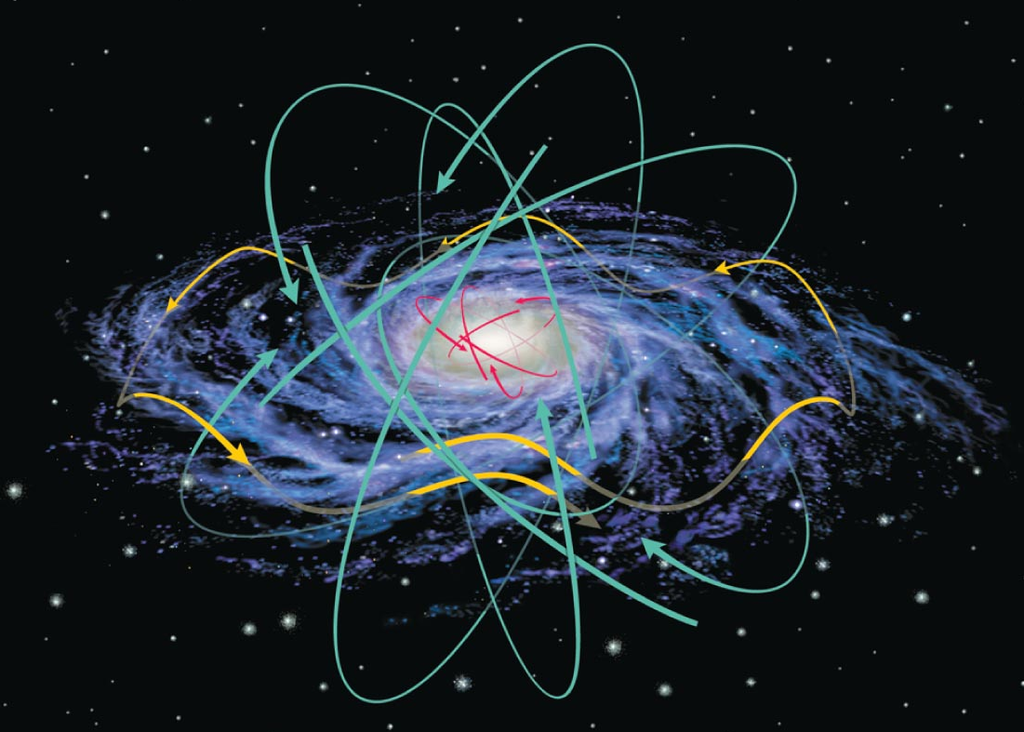
\includegraphics[width=.7\textwidth]{ch15_MW_StarMotions.png}
  \end{center}
  \begin{itemize}
	\item Disk stars move in circular paths + some up-down
	\item Halo stars move in large circles in all directions
	\item Bulge stars have some characteristics of both. More complicated.
  \end{itemize}
\end{frame}

%\begin{frame}{The Scales Don't Lie}
  %\begin{columns}
	%\column{.5\textwidth}
	%\begin{itemize}
	  %\item By observing nearby stars, we know that we orbit the center of the Milky Way at about \SI{220}{\kilo\meter\per\second}
		%\begin{itemize}
		  %\item Gives an orbital period of about 230 million years
		%\end{itemize}
	  %\item We know the distance. We know the period.
		%\begin{itemize}
		  %\item Kepler's Third Law! (Newton's Form)
		  %\item Gives a mass of about \SI{2e41}{\kilo\gram} or 100 billion $M_\odot$!
		%\end{itemize}
	%\end{itemize}
	%\column{.5\textwidth}
	%\begin{block}{Calculation!}
	  %\begin{align*}
		%\frac{P^2}{a^3} &= \frac{4\pi^2}{GM} \\
		%\Rightarrow M &= \frac{4\pi^2 a^3}{G P^2} \\
		%&= \frac{4\pi^2 \left(\SI{2.6e20}{\meter} \right)^3}{(\num{6.67e-11})(\SI{7.258e15}{\second})} \\
		%&= \SI{1.97e41}{\kilo\gram}
	  %\end{align*}
	%\end{block}
  %\end{columns}
%\end{frame}

%\begin{frame}{A Conundrum!}
  %\begin{itemize}
	%\item Planet speeds drop away with distance from the Sun
	%\item We'd expect star speeds to drop away with distance from the center of the galxy
	  %\begin{center}
		%\pause
		%\textcolor{Red}{BUT THEY DON'T!}
	  %\end{center}
	  %\pause
	%\item Implies that all the mass isn't focused at the center, but more spread out
	%\item But there aren't stars in most of those areas!
	%\item Dark Matter?
	  %\begin{itemize}
		%\item Stay tuned for coming chapters!
	  %\end{itemize}
  %\end{itemize}
%\end{frame}

%%\begin{frame}{Reduce, Reuse, Recycle!}
  %%\begin{center}
	%%\includegraphics[width=.7\textwidth]{ch15_stars_lifecycle_full.jpg}
  %%\end{center}
%%\end{frame}

%\begin{frame}{The Milky Way in Various Wavelengths}
  %\url{http://www.chromoscope.net/}
%\end{frame}

\end{document}
